\section{Homework 5}
\subsection{Exercise 4.15}

Relaxation of a boolean LP

A boolean linear program is defined as 
\begin{align}
  \text{minimize} & \quad c^T x \\
  \text{subject to} & \quad Ax \preceq b \\
  & \quad x_i \in \{ 0,1\}, i = 1, \dots, n 
\end{align}
This linear program can be relaxed by replacing the integer constraint with linear inequalities
\begin{align}
  \text{minimize} & \quad c^T x \\
  \text{subject to} & \quad Ax \preceq b \\
  & \quad 0 \leq x_i \leq 1, i = 1,\dots,n
\end{align} 
\subsubsection{Part a}
The optimal value of the LP relaxation is a lower bound on the optimal value. We can use a geometric example to prove this. Since the affine constraints in both the relaxed and original LP form a polyhedron. There are distinct vertex that either do or don't coincide with an integer point. In the event that the polyhedron's vertices land on the integer point, then if the optimal value lies on that vertex, then the optimal value for both the relaxed problem and original problem are equal. In the event that the vertex does not lie on the integer point, then the solution to the relaxed LP is a lower bound on the optimal value of the boolean LP.  \\ \\
The image below illustrates how the vertices lie on integers and therefore the optimal values would be equal. However, if the polyhedron extended out a bit to $(0,0.5),(0.5,0)$ as opposed to $(0,1),(1,0)$ then the relaxed polyhedron would be a strict lower bound.
\begin{figure}[htbp]
  \centerline{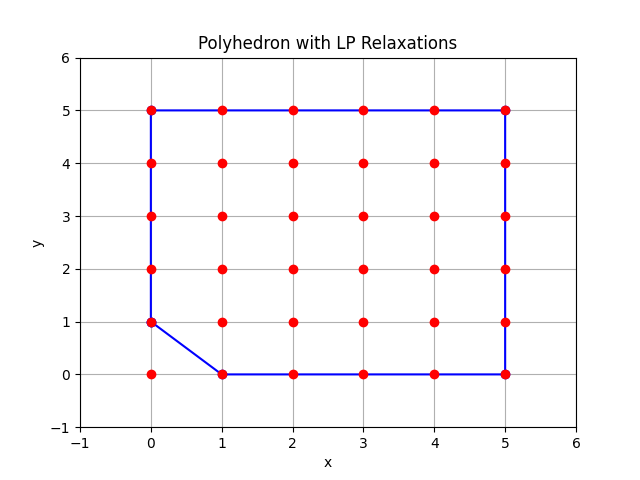
\includegraphics[width=0.50\textwidth]{hw5/lp_relaxed_polyhedron.png}}
  \caption{A polyhedron in $\mathbb{R}^2$ with points at each integer}
  \label{fig:lp_relaxed_polyhedron}
\end{figure} 
\subsubsection{Part b}
This section was also answered in part a. However, the solutions for the relaxation and original problem will coincide whenever the polyhedron created by the given $A$ and $b$ lie on an integer.

\subsection{Exercise 4.60}
\begin{itemize}
  \item $x$: An allocation strategy that dictates the portion of the wealth allocated to each $i$ asset. $x \in \mathbb{R}^n$
  \item $n$: Number of assets
  \item $N$: Number of periods
  \item $W(t-1)$: Amount of wealth at the beginning of period $t$ or end of period $t-1$
  \item $\lambda(t)$: Total return during period $t$. $\lambda(t) = \frac{W(t)}{W(t-1)}$. A random variable with $m$ possible values.
  \item $\frac{1}{N} \sum_{t=1}^{N} \log \lambda(t)$: Growth rate of the investment over $N$ periods.
  \item $m$: Number of deterministic return scenarios.
  \item $\pi_j$: Probability of getting scenario $j$ at any given period. $\pi_j = \textbf{prob}(\lambda(t) = p_j^T x)$
  \item $p_{ij}$: The return for asset $i$ over one period in which scenario $j$ occurs.
\end{itemize}

Our goal here is to maximize our total expected long-term growth rate. First, for my understanding, I am going to derive the formula for the growth rate.
\begin{equation}
  \begin{aligned}
    W(N) = W(0) \prod_{t=1}^{N} \lambda(t) \\
    \frac{1}{N} \log (W(N) - W(0)) = \frac{1}{N} \log \prod_{t=1}^{N} \lambda(t) \\
    = \frac{1}{N} \sum_{t=1}^N \log \lambda(t)
  \end{aligned}
\end{equation}
Now, with this I am going to derive the formula for long term growth rate.

\begin{equation}
  \begin{aligned}
    \lim_{N \to \infty} \frac{1}{N} \sum_{t=1}^N \log \lambda(t) = \mathbb{E}[\log \lambda(t)] \\ 
    = \sum_{j=1}^m \pi_j \log p_j^\top x
  \end{aligned}
\end{equation}

The final optimization problem is:

\begin{align}
  \text{maximize} & \quad \sum_{j=1}^m \pi_j \log p_j^\top x \\
  \text{subject to} & \quad x \succeq 0  \\
  & \quad \textbf{1}^\top x = 1
\end{align}

This question requires that we prove that the above optimization problem is a convex optimization problem. For convention, the problem is turned into

\begin{align}
  \text{minimize} & \quad -\sum_{j=1}^m \pi_j \log p_j^\top x \\
  \text{subject to} & \quad x \succeq 0  \\
  & \quad \textbf{1}^\top x = 1
\end{align}

For this to be a convex problem, the objective function and inequalities must be convex, and the equality constraints must be affine.

Firstly, the objective function is convex:
\begin{itemize}
  \item $p_j^\top x $ is an affine function of the variable $x$
  \item $ \pi_j \log u \text{ with } u = (p_j^\top x)$ is a concave function of the variable $u$, which itself is an affine function of $x$. The function is then multiplied by a non-negative weight which maintains its concavity
  \item $\sum v \text{ with } v = \pi_j \log p_j^\top x$ is a sum of concave functions which is concave.
  \item $- w \text{ with } w = \sum_{j=1}^m \pi_j \log p_j^\top x$ is the negative of a concave function which is convex.
\end{itemize}

Clearly, the inequality is convex as it is the cone $\mathbb{R}^m_{+}$

The equality is indeed affine, therefore the optimization problem is convex!

\subsection{Exercise 5.13}
\subsubsection{Part a}
This part involves finding the lagrange dual of the boolean LP, which we can use to get a lower bound on the original optimization problem.

